\section{Динамические машины состояний}

Для решения задач выбора конкурирующих гипотез -- таких, как разделение
амплитудных импульсов во времени или выбор между гипотезами о
треке частицы,
%в рамках подхода быстрого прототипирования,
целесообразно прибегнуть к высокому уровню общности,
поскольку по мере появления новых детекторов и считывающей аппаратуры,
тестирования и разработки новых методов реконструкции сигналов,
необходимо производить исследование поведения существующих алгоритмов,
производить оптимизацию параметров и часто изменять систему.

Истинная функция отклика подвержена влиянию многих факторов: существенно
зависит от считывающей аппаратуры и изменяется в зависимости от вещества
рабочего объёма детектора.
%Используемая в качестве приближения
%\emph{модельная функция} $f(t,\vec{p})$ --- аппроксимация амплитуды в момент
%времени $t$ праметризуемая параметрами $\vec{p}$
С некоторыми допущениями, для реконструкции
можно применять упрощённую модель или быстрый алгоритм реконструкции с
потерей точности там, где ошибки не так важны как средняя картина
наблюдаемых распределений -- например, при
мониторировании детекторов во время набора данных.
Напротив, для задач анализа целесообразно
стремиться к наиболее правдоподобной модели -- например, для улучшения
разрешения при реконструкции ливней в калориметрах, поскольку
малые амплитуды на периферии ливня приобретают большое значение
в дискриминационных логических схемах.

%Важно отметить, что помимо задачи
%разрешения откликов САЦП, общая постановка задачи справедлива и для
%задачи реконструкции треков, которая в общем формулируется чаще всего
Например, задача реконструкции треков формулируется
как задача минимизации функционала статистики
$\chi^2 = \sum\limits_i (f((t_i,\vec{p}) - r_i)/\sigma_i)^2$ от некоторой (в
общем -- нелинейной, необязательно аналитической) функции параметризации
трека $f(t,\vec{p})$ по отношению к выбранным наборам показаний
координатно-чувствительных детекторов $\vec{r}_i$. При этом
%, как правило, при больших загрузках детекторов,
%типичных для современных экспериментов с большой светимостью,
для разрешения возникающих неоднозначностей применяются различные
алгоритмы отбора: в рамках общей задачи поиска трека~(\emph{track finding})
поиск может производиться по известным пространственным
шаблонам~(\emph{pre-patterning}),
на основе пространственных биекций,
разбиения на KD-дерево, и т.д. ~\cite{MankelTracking, artificial-retina-tracking-lhc}
Такие алгоритмы обычно дают довольно грубое
приближение для более высокоуровневого алгоритма аппроксимации трека,
существенно снижающее набор входных значений по отношению к прямому
комбинаторному перебору.

\subsection{Варианты использования}

Будем подразумевать под \emph{моделью} математическую
функцию $f(x,\vec{p})$, определённую в зависимости от некоторого
аргумента $x_i$ и вектора параметров $\vec{p}$. Целью
\emph{процедуры минимизации} является отыскание таких параметров $\vec{p}$
при которых достигается наилучшее соответствие набору входных данных $y_i$
согласно некоторой метрике.
При этом под программной~\emph{процедурой} в общем, далее мы будем понимать формальный
алгоритм осуществляющий преобразование вектора параметров
модели~$P(\vec{p}_a) = \vec{p}_b$ (т.е. не обязательно
минимизации).
%Символически, можно записать, что для некоторой метрики $\mathbb{M}$
%преобразование заданное процедурой $P$
%т.е. целью процедуры как преобразования $P[\vec{p}_a] \rightarrow \vec{p}_b$
%является отыскание таких $\vec{p}_b$ при которых достигается
%условие~$\text{min}()$

Выделим как минимум следующие основные варианты использования системы,
с точки зрения пользовательского кода, расширяющие исходный
сценарий~\emph{применения процедуры к программной модели}:
\begin{itemize}
    \item Элементарный вариант использования состоит в прямом
    \emph{изменении параметров модельной функции}. Такой этап может быть
    полезен, например, при введении искусственного возмущения в
    линейных алгоритмах минимизации с целью преодоления локальных
    минимумов.
    \item \emph{Применения алгоритма численной минимизации}. Помимо МНК сюда
    относится, например, фильтр Калмана в его различных модификациях,
    и в целом задачи линейного программирования допускающие выражение
    в виде линейно-алгебраических операций над модельной функцией с
    фиксированным набором параметров.
    \item Выбор и \emph{установка начальных значений} параметров $\vec{p}$
    на основе исходной выборки значений $x_i$. Этот вариант
    подразумевает предварительной вычисление начальных приближений
    на основе широкого набора параметров регулирующих поведение
    поисковых алгоритмов.
    \item \emph{Применение процедур к отдельным элементам и подразумеваемая}
    в таком случае \emph{декомпозицию модели} может понадобиться,
    когда с точки зрения численной процедуры минимизации, модель может
    быть тем или иным образом разложена (факторизована) на набор более
    элементарных независимых моделей, к каждой из которых необходимо
    применить определённый набор процедур. Например: аппроксимация
    функции отклика для значительно разнесённых во времени пиков,
    аппроксимация трека частицы на линейных участках в отсутствии
    магнитного поля, и т.д.
    \item Для \emph{сопоставления результатов} аппроксимации между
    конкурентными методами посредством определённой метрики (в частности,
    выбор наилучшей гипотезы о треке на основании $\chi^2$), необходима
    соответствующая процедура, делегирующая выполнение альтернативным процедурам.
    \item В тех случаях, когда метрика не может быть определена для
    моделей, и основным результатом является логическое условие применимости
    процедуры, целесообразно выделить вариант использования перебирающий
    процедуры до тех пор, пока очередной вариант не будет
    выполнен успешно (\emph{выбор подходящей модели}).
    \item Наконец, \emph{выбор или замена модельной функции} в рамках
    такого уровня общности тоже представляет собой вариант использования.
\end{itemize}

\begin{figure}
    \centering
    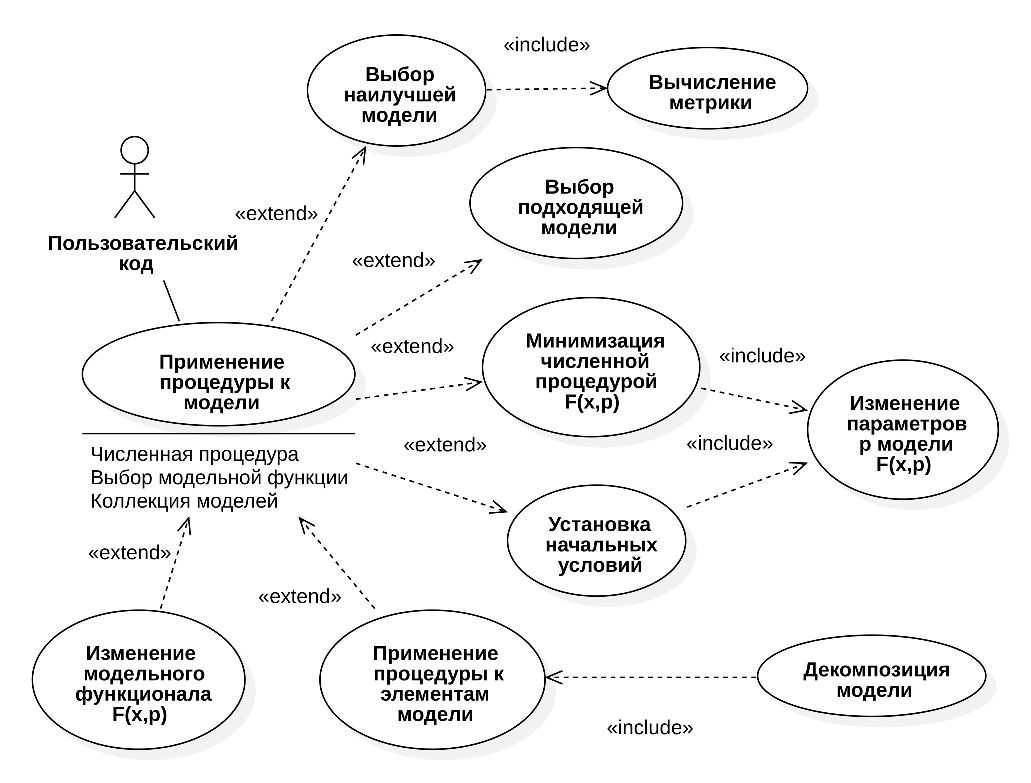
\includegraphics[width=0.95\linewidth]{images/umff-usecase-diagram-02.eps}
    \caption{Диаграмма вариантов использования программной библиотеки для
    решения задач численной минимизации с расширенной логикой (ветвление,
    сопоставление, перебор).}
    \label{fig:umff-usecases}
\end{figure}

Рисунок \ref{fig:umff-usecases} иллюстрирует отношения между перечисленными вариантами
использования.

\subsection{Компоненты машины конечных состояний}

Описанная структура вариантов использования подразумевает наличие по крайней мере
следующих элементов обобщённого поведения:
\begin{itemize}
    \item Составная процедура содержащая набор более простых процедур,
    делегирующая выполнение этому набору, и завершающаяся результатом
    отобранным согласно некоторому правилу (\emph{competing}).
    \item Составная процедура осуществляющая декомпозицию модели в тех случаях,
    когда модель это позволяет, инкапсулирующая набор более простых процедур,
    и применяющая этот набор по отдельности к каждому элементу
    декомпозиции~(\emph{breakdown}).
    \item Последовательность процедур в которой последующая применяется только
    в том случае, если текущая завершилась не успешно
    (\emph{fallback}).
    %Рисунок \ref{fig:fallback-example} содержит
    %пример машины конечных состояний, в которой применение процедуры
    %делегируется, а валидация выполняется самим элементом.
\end{itemize}

Этот базовый набор логических элементов позволяет конструировать сложные
алгоритмы, опираясь на более элементарные, порождая машину
конечных состояний, в которой состояниям отвечает модель ($m_i:=f(x_i,\vec{p})$),
а переходам соответствует процедура $P(\vec{p}_a) = \vec{p_b}$.

Техническое описание и спецификации вынесены в приложение~\ref{appendix:fsm-machine-prog}.

\subsection{Восстановление амплитудных сигналов}

На рисунке~\ref{fig:sadc-wf-fitting-example} приведён пример
восстановленного отклика ячейки электромагнитного калориметра от двух
импульсов слабо разнесённых во времени. Пунктирной линией
с коротким штрихом
изображён график конечно-разностной аппроксимации первой производной
по точкам сигнала, сплошными серыми линиями изображён результат
подгонки -- для отдельных импульсов и их восстановленная сумма.
Пунктирная линия с длинным штрихом отвечает начальным условиям.

\begin{figure}[ht]
    \centering
    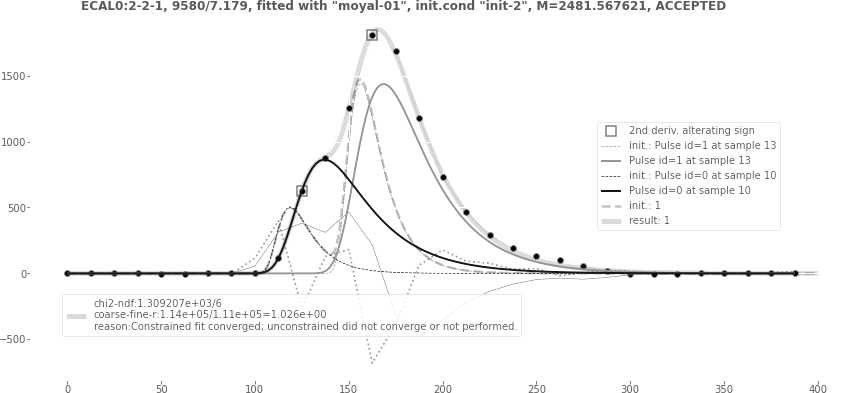
\includegraphics[width=0.99\linewidth]{images//illustrative/waveform-fit-result-example.png}
    \caption{Пример восстановления сигнала от двух частиц с малой временным
    интервалом; время в наносекундах против амплитуды в относительных единицах}
    \label{fig:sadc-wf-fitting-example}
\end{figure}

Этот случай имеет большое значение в отношении физической картины,
поскольку подобную сигнатуру часто дают мюоны от
распадающихся в голове канала
пионов $\pi^{\pm} \rightarrow \mu^{\pm} \nu_\mu$ 
и каонов $K^{\pm} \rightarrow \mu^{\pm} \nu_\mu$,
или мюонные пары от реакций $\gamma Z \rightarrow Z \mu^{+}\mu^{-}$.

Наивный алгоритм построенный на выделении абсолютного максимума
не способен обнаружить первый импульс от слабоэнергетической частицы.
Более того, первый импульс вообще не даёт максимума. 

Второй пик распознаётся специализированным алгоритмом отыскания
импульсов, опирающимся на сигнатуру чередования роста и спада
функции. Аппроксимация моделью затем производится с учётом
индивидуальных особенностей ячейки, поскольку в общем случае
подгонка параметров модели в данной картине допускает неоднозначность
результатов. Кроме того, из-за присутствующей неоднозначности
весьма вероятна сходимость процедуры подгонки к локальному минимуму,
что решается посредством одновременного рассмотрения
нескольких конкурирующих гипотез.
